\documentclass[journal]{IEEEtran}

% *** GRAPHICS RELATED PACKAGES ***
\ifCLASSINFOpdf
	\usepackage[pdftex]{graphicx}
	\graphicspath{{images/}}
	% \DeclareGraphicsExtensions{.pdf,.jpeg,.png}
\else
	\usepackage[dvips]{graphicx}
	\graphicspath{{images/}}
	% \DeclareGraphicsExtensions{.eps}
\fi

% *** SUBFIGURE PACKAGES ***
\ifCLASSOPTIONcompsoc
  \usepackage[caption=false,font=normalsize,labelfont=sf,textfont=sf]{subfig}
\else
  \usepackage[caption=false,font=footnotesize]{subfig}
\fi

% correct bad hyphenation here
\hyphenation{op-tical net-works semi-conduc-tor}

\newcommand{\fref}[1]{\figurename \ref{#1}}

\begin{document}

% paper title
\title{Full Custom DAC Design Coursework}

% author names and IEEE memberships
\author{Yubo~Zhi (yz4116)}

% The paper headers
\markboth{Full Custom DAC Design Coursework}%
{Full Custom DAC Design Coursework}

% make the title area
\maketitle

\begin{abstract}
This coursework is about design a Digital to Analogue Converter (DAC) using full custom CMOS process. The design specifications was successfully achieved by using capacitor array approach. A compact layout was also designed using various techniques.
\end{abstract}

\section{Introduction}
\IEEEPARstart{D}{igital} to Analogue Converter is an essential interface component heavily used in modern technology. It generates an analogue voltage signal based on its digital inputs. In this coursework \cite{cw}, a DAC with 8-bit precision and serial data input was designed using full custom CMOS process, so that it can potentially be used as a component in integrated circuits.
 
\hfill \today

\section{System Overview}

There are 3 possible topologies for this coursework \cite{cw}, R-2R Ladder based, capacitor array based or current steering based \cite{dac}.

It would be quit difficult to match resistors for R-2R Ladder topology. Moreover, parasitic resistances of MOSFETs may significantly affect the accuracy.

For capacitor array and current steering topology, the size of capacitors or the width of MOSFETs need to be doubled for each bit. For the specified 8-bit resolution, that would require about 512 times the layout area of a unit component. The current steering topology will also be affected by MOSFET parasitic resistances, whereas the capacitor array topology will only be affected by parasitic capacitances, which can be insignificant compare to the unit capacitor for an 8-bit DAC.

Further more, a split capacitor can be used in the capacitor array topology. By splitting the capacitors to 2 groups of 4 bits, only about 32 times the layout area of a unit capacitor would be needed. Common centroid and dummy devices layout techniques can also be used to improve component matching. By not having a continuous current flow comparing to the other 2 topologies, it would have a lower static power consumption. Therefore the capacitor array approach with a split capacitor was used in this coursework.

\fref{fig_system} shows the system block diagram of the proposed DAC design.

\begin{figure}[!t]
	\centering
	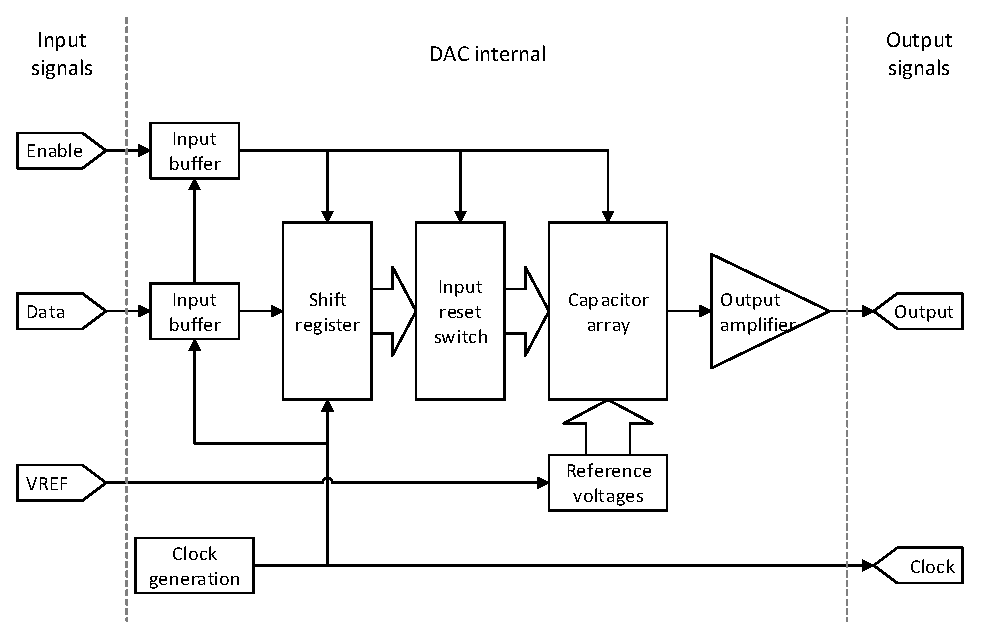
\includegraphics[width=\columnwidth]{System}
	\caption{System block diagram}
	\label{fig_system}
\end{figure}

Data clock is generated inside the DAC module by a 10MHz ring oscillator.

Serial data input and enable signal are captured by 2 D-type flip-flops (DFF) at raising edge of the clock. These DFFs are used to avoid metastability issues, when inputs are changing at the same time the clock signal is rising. They will also hold the input for the rest of the clock cycle.

The serial data input then enters an 8-bit shift register. It will register each bit and output as an 8-bit parallel interface for the capacitor array. The clock to shift register was gated by the enable signal, so it will hold the output when enable is not asserted.

The capacitor array consists of binary weighted capacitors. It works by charge redistribution that happens when different capacitors are hold at different voltage levels, with another terminal connected together. Therefore, it is essential to always release the existing charges on the capacitors before every conversion. Thus another input switch that connects the capacitor array inputs to ground during reset is needed.

According to specification, the output range should be from $0.4 V$ up to $1.4 V$. Therefore, voltage references are needed to biasing the capacitor array, so that it works at the specified voltage range. Overall gain and offset errors can also be compensated by adjusting the voltage references.

The output impedance of the capacitor array is very high, as there are only capacitors connected. Therefore, an output amplifier is required.

\section{Circuit Implementation}

\subsection{Clock generation}

The 10MHz digital clock is generated by using a ring oscillator. \fref{fig_ringosc} shows the schematic and layout design of the ring oscillator. Long channel MOSFETs are used to reduce oscillation frequency. 2 inverters are used to amplify and shape the output. Simulations are used to tune MOSFET parameters.

The spacing between N+ implant and the cell boundary is $0.2 \mu m$, half the design rule for N+ implant spacing ($0.4 \mu m$), same as others. It also has the same cell height of $8 \mu m$ as other digital blocks, so it can be placed tightly with other digital blocks.

\begin{figure*}[!t]
	\centering
	\subfloat[Schematic]{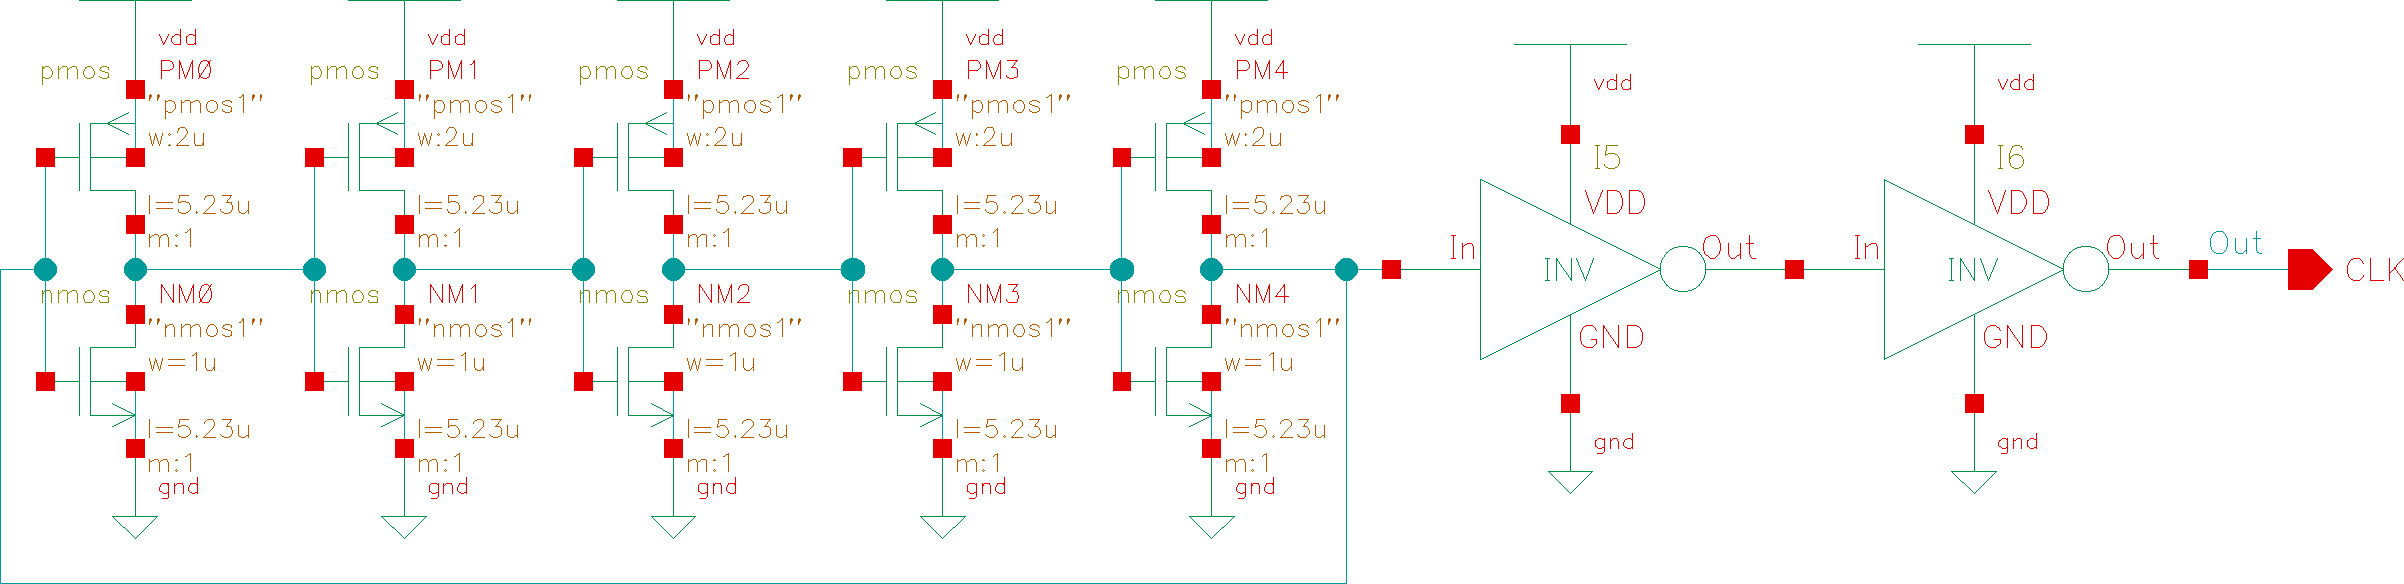
\includegraphics[width=\columnwidth]{ringosc_sch}%
	\label{fig_ringosc_sch}}
	\hfil
	\subfloat[Layout]{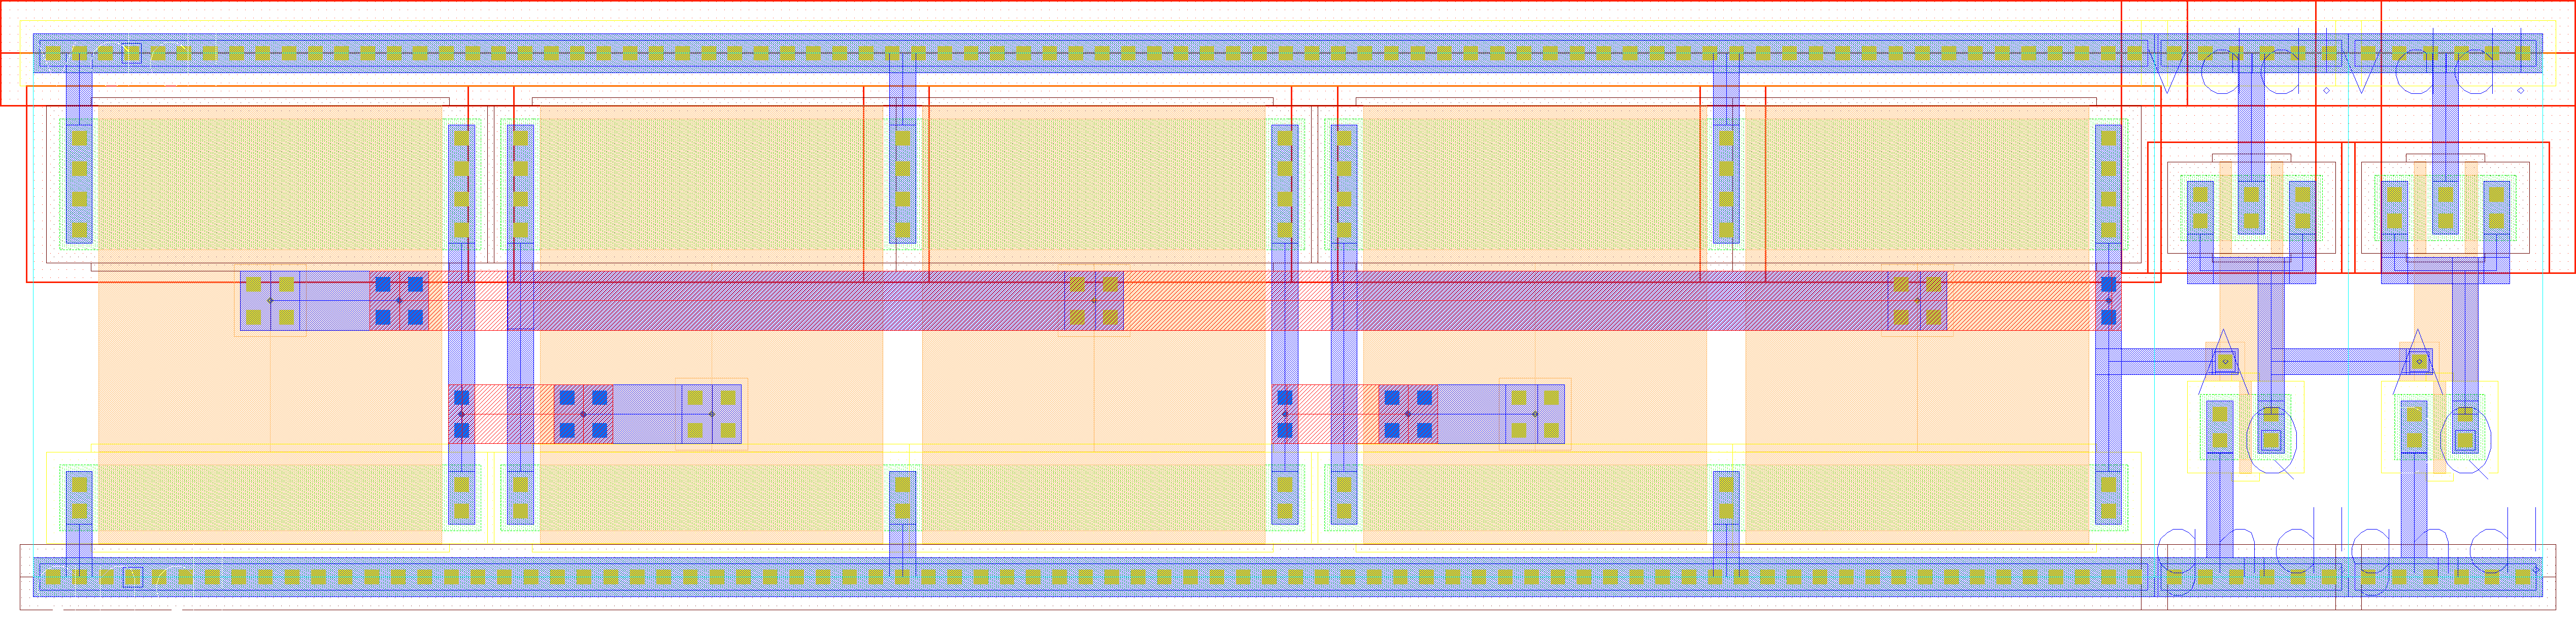
\includegraphics[width=\columnwidth]{ringosc_lay}%
	\label{fig_ringosc_lay}}
	\caption{Ring oscillator design}
	\label{fig_ringosc}
\end{figure*}

\subsection{Digital blocks}

\subsubsection{Shift register}

The shift register was realised by chaining 8 D-type flip-flops. Special D-type flip-flops that have inverted clock input and both inverting and non-inverting outputs was used, to remove the need of a few inverters.

\fref{fig_clock} shows the clock gating of the shift register. The clock input to the NAND is inverted, to prevent potential clock glitch that might happen when clock rises then buffered enable signal falls a bit later. Because of propagation delay, the clock signal to shift register will be delayed related to the clock generator. Therefore, it would be better to sample the buffered data input at falling edge, hence the inverted clock input.

\begin{figure}[!t]
	\centering
	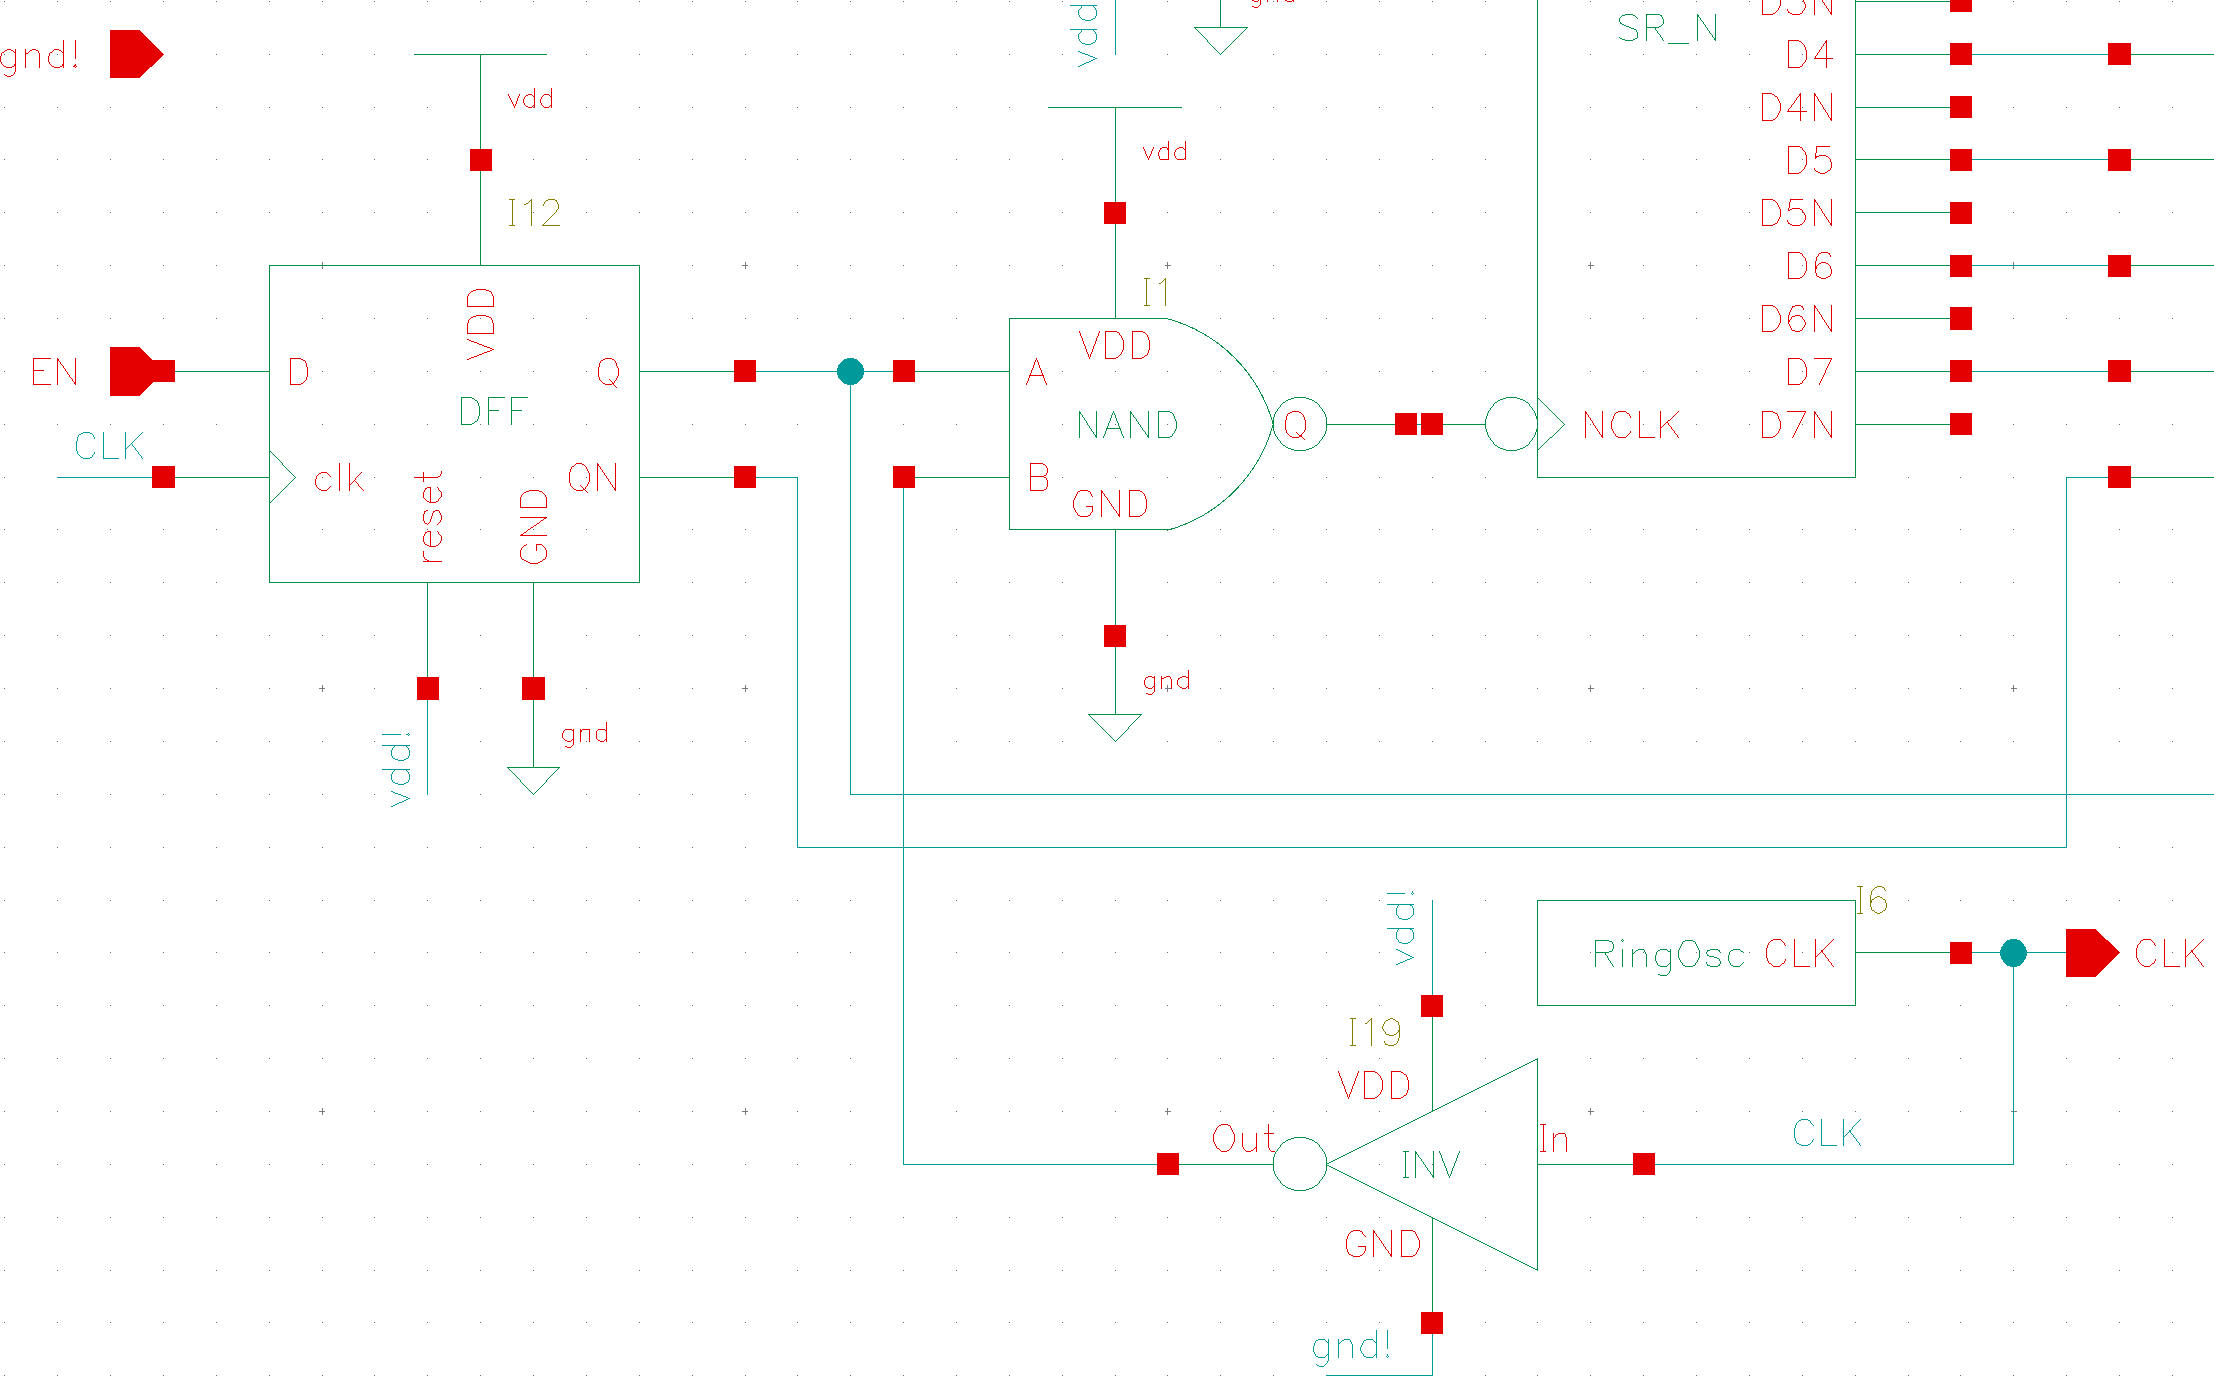
\includegraphics[width=\columnwidth]{clock}
	\caption{Shift register clock gating}
	\label{fig_clock}
\end{figure}

\subsubsection{Input reset switches}

The input switches are simply 8 NANDs. The input of capacitor array drives MOSFETs arranged like an inverter, thus the output of this stage should be inverted. Inverted enable signal come from input buffer was used, so the output will be high when enable is asserted. Also using the inverted output from shift register, simple NANDs are sufficient.

\subsection{Capacitor array}

\fref{fig_cap_split} shows a 6-bit charge-scaling DAC realised using capacitor array with split capacitor.

%\begin{figure}[!t]
%	\centering
%	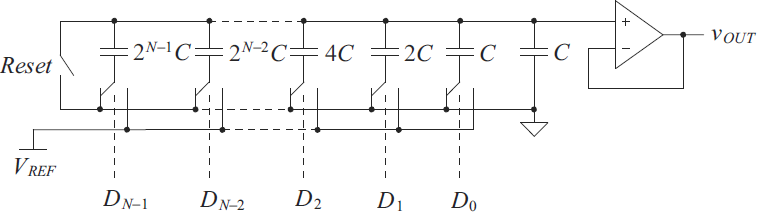
\includegraphics[width=\columnwidth]{cap_basic}
%	\caption{Charge-scaling DAC (adapted from \cite{cap_dac})}
%	\label{fig_cap_basic}
%\end{figure}

\begin{figure}[!t]
	\centering
	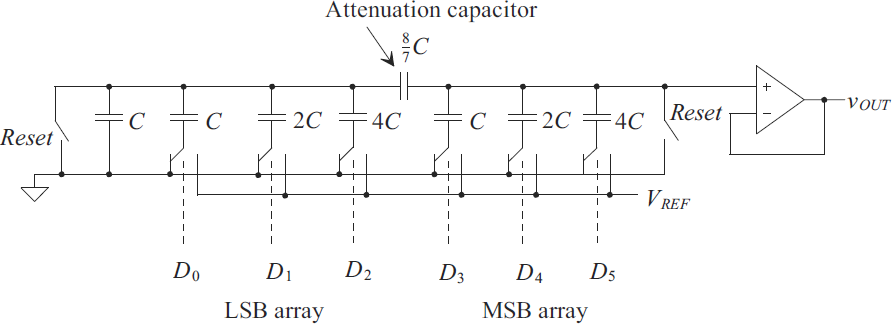
\includegraphics[width=\columnwidth]{cap_split}
	\caption{A charge-scaling DAC using split array (adapted from \cite{cap_dac})}
	\label{fig_cap_split}
\end{figure}

After initial discharge, by having binary-weighted capacitors connected to either VREF or GND, the capacitors will be charged, with output node have a voltage proportional to charge distribution, hence the name "charge-scaling". There are no static current flow in the capacitor array, therefore very power efficient. It is very sensitive to parasitic capacitances, so the capacitors need to be big enough to overcome them.

%\fref{fig_cap_sch} shows the actual schematic of capacitor array design, including dummy capacitors.

%\begin{figure}[!t]
%	\centering
%	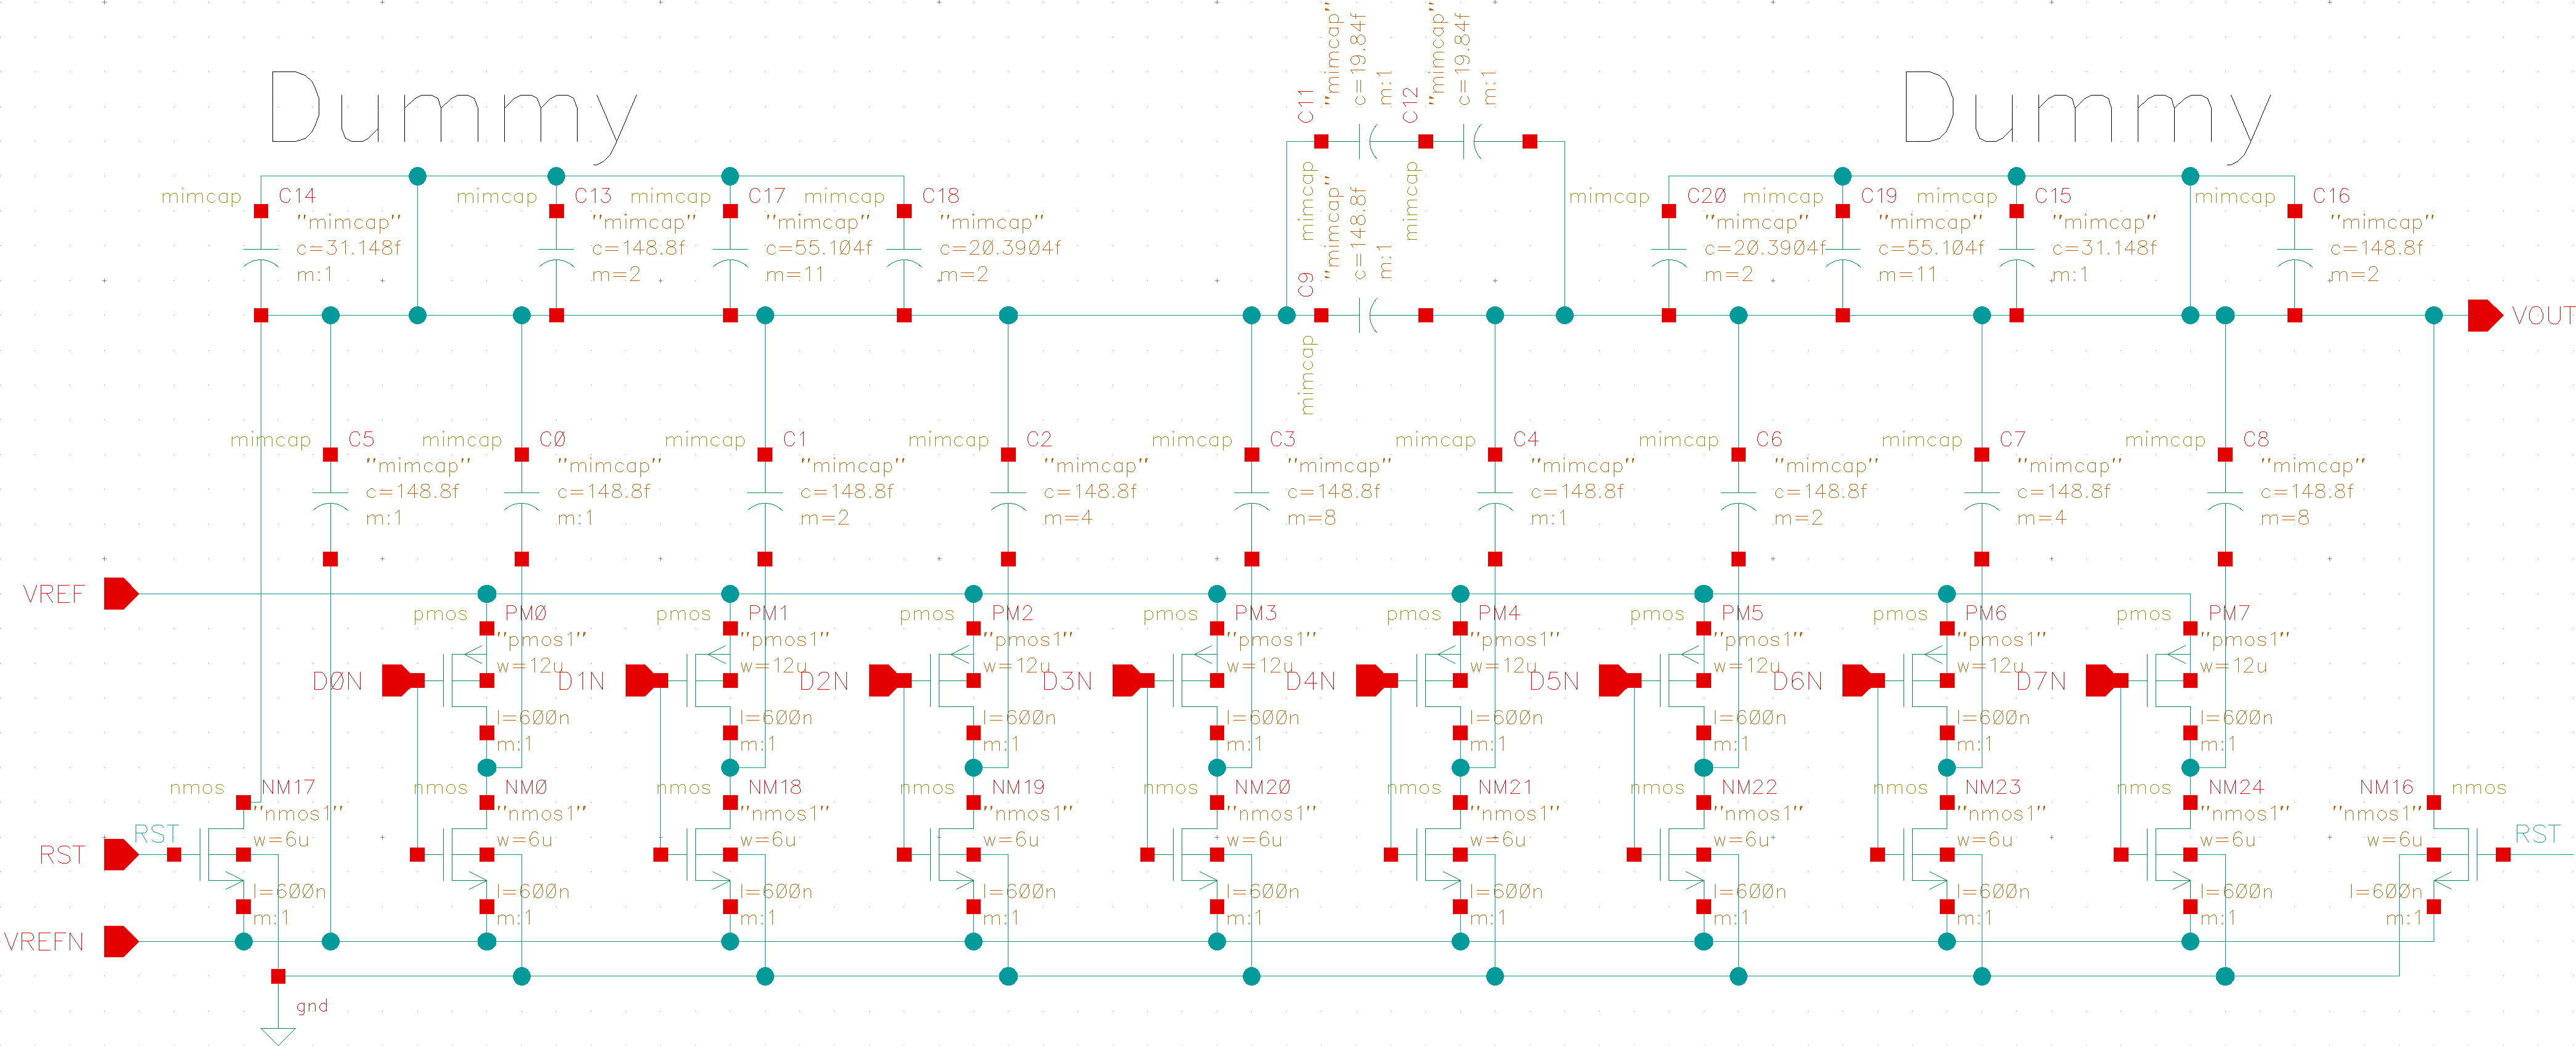
\includegraphics[width=\columnwidth]{cap_sch}
%	\caption{Schematic design of capacitor array}
%	\label{fig_cap_sch}
%\end{figure}

\fref{fig_cap_lay} shows the actual layout design of the capacitor array. M and L capacitors corresponding to capacitors used in most significant bits and least significant bits respectively, while S capacitors form the split capacitor. Dummy capacitors (D) were also added for better matching around the edge.

\begin{figure}[!t]
	\centering
	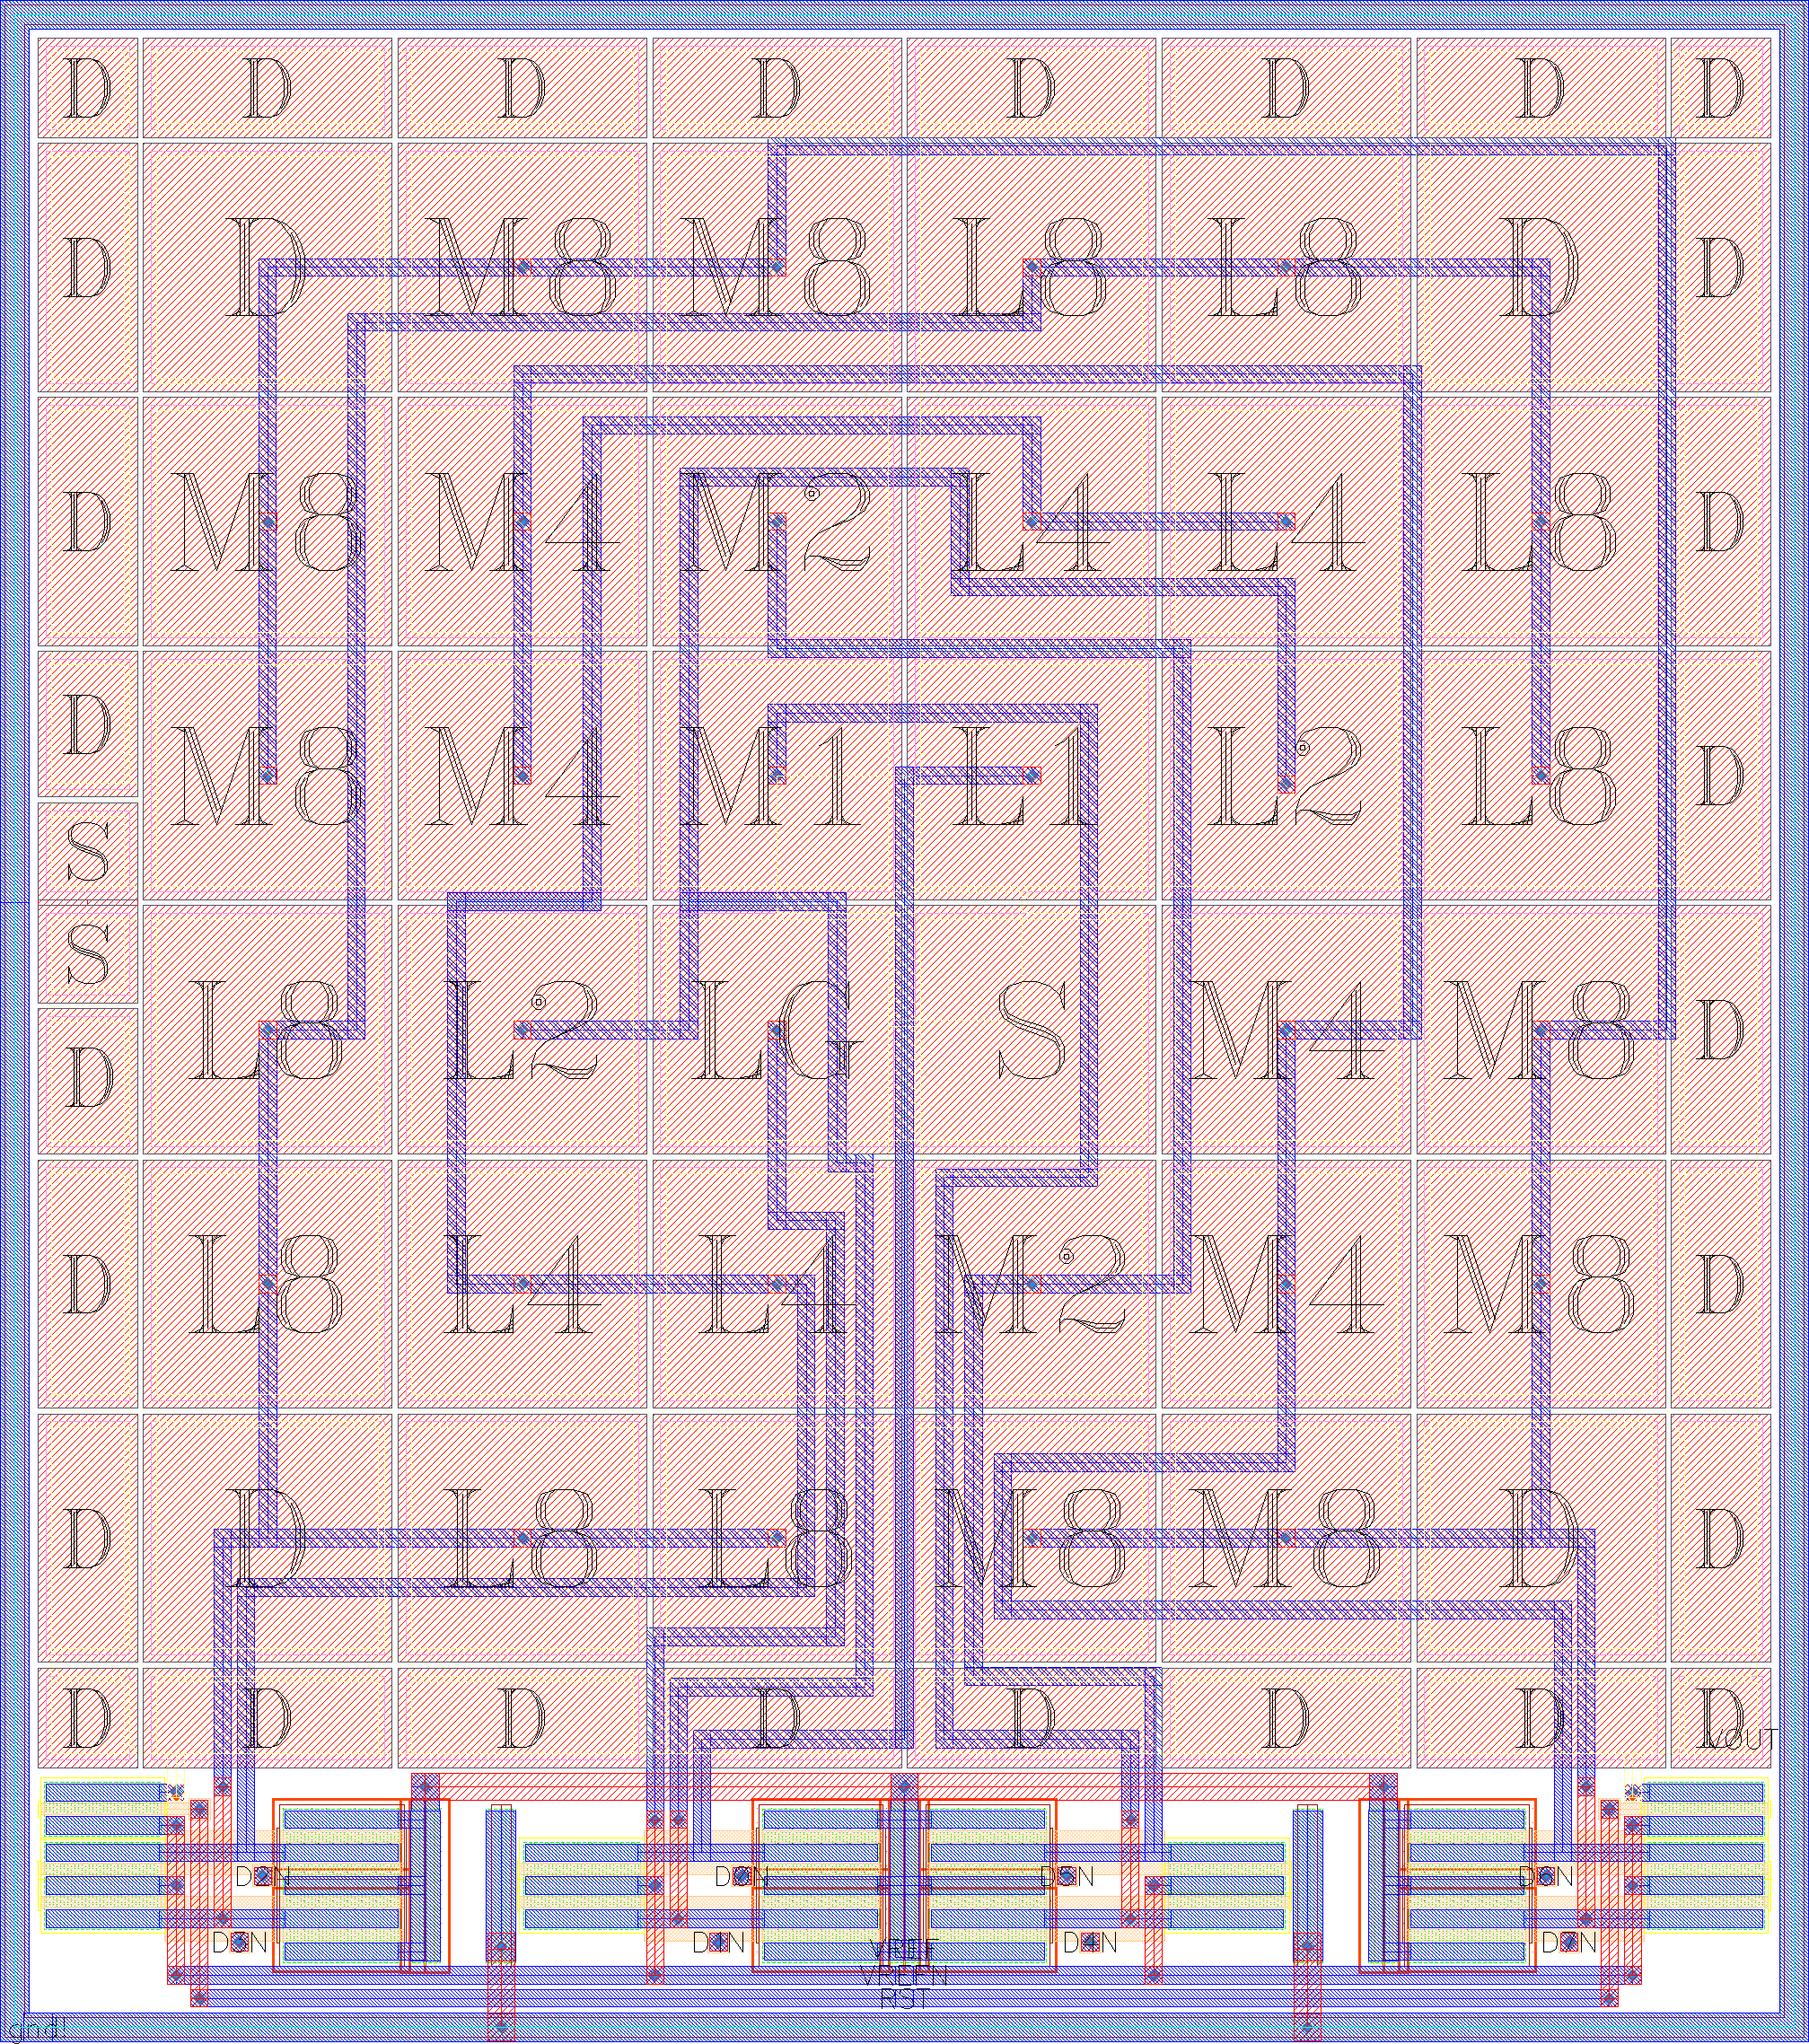
\includegraphics[width=2.5in]{cap_lay_4x}
	\caption{Lay design of capacitor array}
	\label{fig_cap_lay}
\end{figure}

The capacitors are placed in a common centroid configuration, as indicated by the text on each unit capacitor. In this arrangement, component value variation caused by first order gradient on wafer will be cancelled out.

\subsection{Voltage references}

\subsection{Output amplifier}

Circuit theory of operation.

Annotated schematics and layout.

Discussion of advanced issues considered / addressed and unique features and limitations of your design.

\section{Simulated Results}

Results and Interpretation / discussion.

Description of the test strategy used and a schematic test bench.

Simulation results to demonstrate that the circuit operates as expected.

\section{Conclusion}

Table of technical specifications.

% references section
\begin{thebibliography}{1}

\bibitem{IEEEhowto:kopka}
H.~Kopka and P.~W. Daly, \emph{A Guide to \LaTeX}, 3rd~ed.\hskip 1em plus
  0.5em minus 0.4em\relax Harlow, England: Addison-Wesley, 1999.

\end{thebibliography}

% that's all folks
\end{document}
